\documentclass[12pt]{article}

\usepackage{sbc-template}

\usepackage{graphicx,url}
\usepackage[brazil]{babel}
\usepackage[utf8]{inputenc}
\usepackage[T1]{fontenc}
\usepackage[hidelinks]{hyperref}
\usepackage{booktabs}


\sloppy

\title{Smartphone-Based Recognition of Human Activities and Postural Transitions}

\author{Bruno M. Dobrovolski\inst{1}, Eduardo A. Schmoller\inst{1}}

\address{Departamento Acadêmico de Informática -- Universidade Tecnológica Federal do Paraná\\
	Pato Branco -- PR -- Brasil	
	\email{\{brunod,schmoller\}@alunos.utfpr.edu.br}
}

\begin{document} 

\maketitle

%\begin{abstract}
%  This meta-paper describes the style to be used in articles and short papers
%  for SBC conferences. For papers in English, you should add just an abstract
%  while for the papers in Portuguese, we also ask for an abstract in
%  Portuguese (``resumo''). In both cases, abstracts should not have more than
%  10 lines and must be in the first page of the paper.
%\end{abstract}
%
%\begin{resumo}
%  Este meta-artigo descreve o estilo a ser usado na confecção de artigos e
%  resumos de artigos para publicação nos anais das conferências organizadas
%  pela SBC. É solicitada a escrita de resumo e abstract apenas para os artigos
%  escritos em português. Artigos em inglês deverão apresentar apenas abstract.
%  Nos dois casos, o autor deve tomar cuidado para que o resumo (e o abstract)
%  não ultrapassem 10 linhas cada, sendo que ambos devem estar na primeira
%  página do artigo.
%\end{resumo}

\section{Introdução}

%	Exemplo artigo: \url{https://www.elen.ucl.ac.be/Proceedings/esann/esannpdf/es2013-11.pdf}\\

	Este trabalho apresentará resultados da aplicação de métodos de aprendizado de máquinas na predição de movimentos humanos. Foram implementados os seguintes métodos de aprendizado: KNN, Perceptron e SVM. 
	
	Os dados para base para treinamento e teste foram obtidos de \cite{Dua:2017}. Essas informações são referente a sensores de um dispositivo móvel Galaxy Samsung S2. O \textit{smartphone} foi mantido junto ao corpo dos voluntários em atividades de: Levantar, sentar, deitar, caminhar, subir escadas e descer escadas. Os testes foram executados com 30 voluntários e os dados coletados através dos sensores do smartphone, acelerômetro de 3 eixos e giroscópio de 3 eixos.
	
	Os dados obtidos dos sensores foram pré-processados com a aplicação de filtros para remoção de ruídos, amostrados em intervalos constantes de tempo e normalizados. Também foram segmentados separando cada um dos 3 eixos e calculando várias informações estatísicas (totalmente descritas em cite{Dua:2017}), como média, desvio padrão, máximo, mínimo, entre outras, totalizando 561 características.Cada conjunto de dados que representa os movimentos recebeu uma identificação. O conjunto de características e de idenficações (\emph{label}) são entradas para os algoritmos de classificação.
	
	Como forma de validação do processo de aprendizado, o conjunto de dados de entrada foi dividido em dois subconjuntos denominados conjunto de treino e conjunto de testes. O conjunto de treino é utilizado no processo de treinamento, após o processo de treinamento o conjunto de testes é classificado e os resultados são comparados com as resultados esperados.
	
	Ainda, os algorítimos foram alterados através da redução de dimensionalidade com o uso do método PCA. Como esse método não entrega um resultado ótimo, foi necessário variar o número de componentes para encontrar a melhor combinação.

	Como métrica para a determinação da qualidade do processo de aprendizados foram utilizadas a acurácia da predição e utilização do \emph{kappa score}. O \textit{kappa score} funciona como uma validação do resultado apresentado pela acurácia, visto que ele considera em seu calculo os resultados falso-positivos e falso-negativos, colocando peso em cada uma das características. 

\section{Revisão}

	Esta seção apresenta os métodos aplicados para a classificação dos movimentos.

\subsection{Perceptron}

%	\url{http://ml.informatik.uni-freiburg.de/former/_media/documents/teaching/ss09/ml/perceptrons.pdf}

	Separador linear através de uma função de \emph{threshhold}, reta esta que é definida através de pesos. O treinamento de um perceptron consiste na entrada de um conjunto de casos e calcular a saída para cada caso, após cada entrada os pesos são ajustados de forma a minimizar o erro na saída, o erro é definido como a diferença entre a saída e a saída esperada, não existe erro caso a saída e a saída esperada sejam iguais.
	
	Perceptron de uma única camada apenas separam problemas lineares, para a classificação de classes que não sejam separáveis linearmente é necessário um perceptron de múltiplas camadas.
	
\subsection{KNN}

	KNN algoritmo simples que realiza o aprendizado de todas as entradas e classifica as novas entradas com base na similaridade dos casos já aprendidos. Ao realizar a classificação de uma nova entrada é retornado \emph{k} vizinhos mais próximos, classificação se dá pela maioria dos vizinhos.
	

\subsection{SVM}

	SVM é um classificador definindo a separação entre as classes através de um hiperplano, a entrada são dados com \emph{labels} e a saída é um hiperplano ótimo para categorização de novas entradas. Em duas dimensões o hiperplano é representado através de uma reta que divide o plano em duas partes.
	
\subsection{PCA}

	Redutor de dimensionalidade selecionando as principais componentes, entre as formas de encontrar as componentes principais é buscar as projeções que maximizem a variança.
	
\subsection{Testes Estatísticos}

	Testes estatísticos são utilizados para validação de hipóteses usando dados amostrais para decidir sobre a validade da hipótese.
	
	Cenários típicos de uso de testes estatísticos em métodos de aprendizado: adição de etapas de processamento, comparar diversos algoritmos, validação de capacidade de generalização de um classificador. O principio básico é a formulação de hipóteses e decidir se os dados mostram alguma evidencia para rejeição da hipótese.
	
%	\url{http://citeseerx.ist.psu.edu/viewdoc/download?doi=10.1.1.558.7319&rep=rep1&type=pdf}\\
%	\url{https://ai.vub.ac.be/sites/default/files/4.\%20Hypothesis\%20Testing.pdf}\\
%	\url{https://www.cl.cam.ac.uk/teaching/1617/MLRD/slides/slides4.pdf}\\
%	\url{http://www.public.asu.edu/~huanliu/dmml_presentation/T-test.pdf}

	\subsubsection{Validação Cruzada}
	
%		\url{https://www.analyticsvidhya.com/blog/2018/05/improve-model-performance-cross-validation-in-python-r/}\\
%		\url{https://towardsdatascience.com/cross-validation-in-machine-learning-72924a69872f}\\
%		\url{https://www.kaggle.com/dansbecker/cross-validation}\\
%		\url{https://www.researchgate.net/profile/Ron_Kohavi/publication/2352264_A_Study_of_Cross-Validation_and_Bootstrap_for_Accuracy_Estimation_and_Model_Selection/links/02e7e51bcc14c5e91c000000.pdf}\\
%		\url{http://scikit-learn.org/stable/modules/model_evaluation.html}
		
		Validação cruzada é uma técnica que consiste em reservar uma parte do conjunto de dados para serem utilizados para testes após a etapa de treinamento.
		
		Exemplos de métodos para validação cruzada: \emph{HoldOut} (dividir em treino e teste), \emph{K-fold} (k sub conjuntos de treino e teste), \emph{Stratified K-Fold} (cada conjunto contem aproximadamente a mesma porcentagem de amostras de cada classe que o conjunto completo), \emph{Leave-P-Out} (em um conjunto de n casos então n-p serão utilizados para treino e p casos para teste).
		
	\subsubsection{Matriz de Confusão}
	
		\url{http://www2.cs.uregina.ca/~hamilton/courses/831/notes/confusion_matrix/confusion_matrix.html}\\
		
	\subsubsection{Kappa Score}
	
		\url{https://www.ncbi.nlm.nih.gov/pmc/articles/PMC3900052/}\\
		\url{http://www.pmean.com/definitions/kappa.htm}\\
		\url{http://www.statisticshowto.com/cohens-kappa-statistic/}\\
		\url{https://academic.oup.com/ptj/article/85/3/257/2805022}
		
\section{Resultados}

	\begin{figure}[!htb]
	\centering
	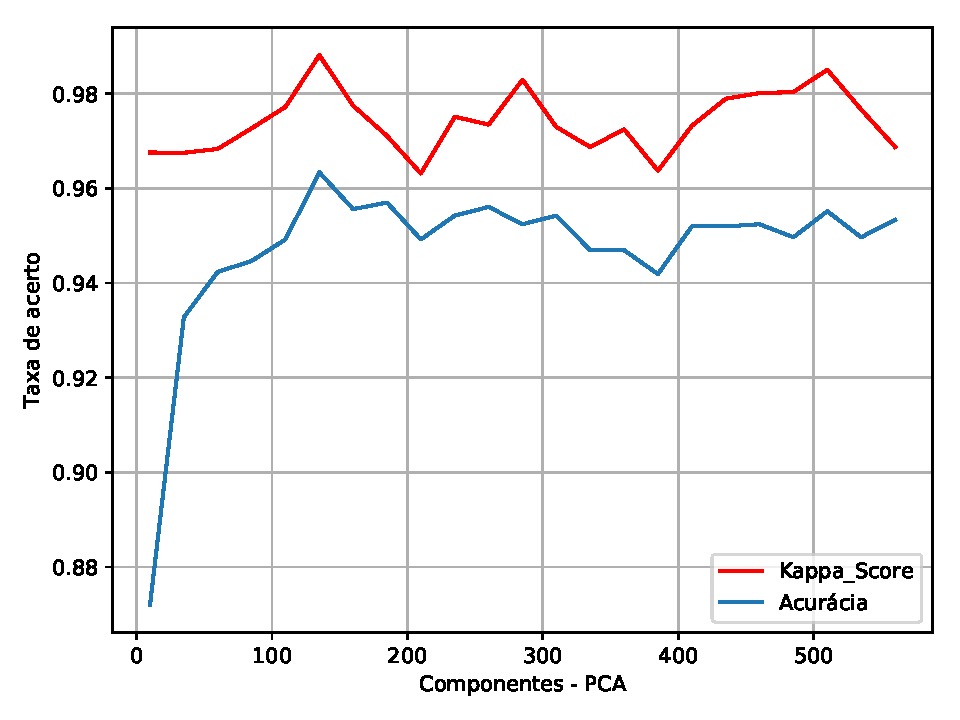
\includegraphics[width=.5\textwidth]{knn_pca_quadratic.pdf}
	\caption{Acurácia e Kappa score KNN}
	\label{fig:knnpcaquadratic}
	\end{figure}

\begin{table}[ht]
	\centering
	\caption{Resultados}
	\label{table:resultados}
	\smallskip
	\begin{tabular}{|l|c|c|}
		\hline
		Método& Acurracia & Kappa Score\\[0.5ex]
		\hline
		&&\\[-2ex]
		KNN & $0.94$ & $0.93$\\[0.5ex]
		\hline
		&&\\[-2ex]
		Perceptron & $0.96$ & $0.96$\\[0.5ex]
		\hline
		&&\\[-2ex]
		SVM & $0.92$ & $0.91$\\[0.5ex]
		\hline
		&&\\[-2ex]
		KNN + PCA & & \\[0.5ex]
		\hline
		&&\\[-2ex]
		Perceptron + PCA & & \\[0.5ex]
		\hline
		&&\\[-2ex]
		SVM + PCA & & \\[0.5ex]
		\hline
	\end{tabular}
\end{table}

\section{Conclusões}
	...

\bibliographystyle{sbc}
\bibliography{sbc-template}

\end{document}
